\section{Problem (5)}
	A elevator cab that weighs $8800 \ lb$ moves upward. What is the tension in the cable if the cab's speed is:

	\subsection{Question (a)}
		Increasing at a rate of $3.8 \ ft/s^{2}$?

		\textbf{R:} \newline

		\begin{figure}[H]
			\begin{center}
				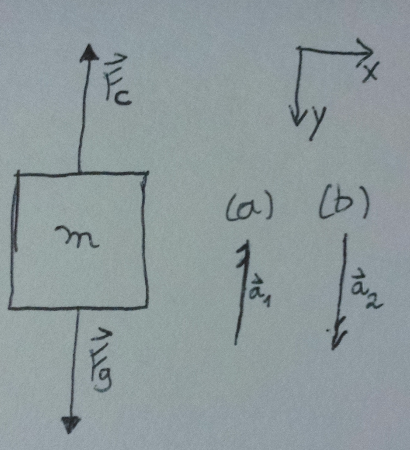
\includegraphics[scale=0.7]{hw5_problem5_fbd}
				\caption{Free-Body Diagram (Problem 5)}
				\label{fig:hw5_problem5_fbd}
			\end{center}
		\end{figure}

		\begin{align}
			m = \ &\frac{8800 \ lb}{32.2 \ ft/s^{2}} = 273.2 \ sl& \notag
		\end{align}

		Newton's $2^{nd}$ Law:
		\begin{align}
			\sum F_{y} = \ &ma_{y}& \notag \\
			F_{c} - F_{g} = \ &(273.2 \ sl)\left( 3.8 \ ft/s^{2}\right)& \notag \\
			F_{c} = \ &(273.2 \ sl)\left( 3.8 \ ft/s^{2}\right) + (8800 \ lb)& \notag \\
			F_{c} = \ &(1038.2 \ lb) + (8800 \ lb) = 9838.2 \ lb&
		\end{align}

	\subsection{Question (b)}
		Decreasing at a rate of $2.9 \ ft/s^{2}$?

		\textbf{R:} \newline
		
		Newton's $2^{nd}$ Law:
		\begin{align}
			\sum F_{y} = \ &ma_{y}& \notag \\
			F_{c} - F_{g} = \ &(273.2 \ sl)\left( - 2.9 \ ft/s^{2}\right)& \notag \\
			F_{c} = \ &(273.2 \ sl)\left( - 2.9 \ ft/s^{2}\right) + (8800 \ lb)& \notag \\
			F_{c} = \ &(8800 \ lb) - (792.3 \ lb) = 8007.7 \ lb&
		\end{align}
